\subsubsection{13.02.2016}
\textit{\textbf{Time frame:}} 16:00-21:30 

The axis on the winch was changed on a shorter one, which wouldn't interfere with the cover of the bucket.

The chain gears on the winch were moved closer to the motors in order to make the mechanism more reliable.

There were added new segments to the front brush in order to enlarge the collecting area.

It was also installed the protection which would prevent debris from getting under the wheels (figure \ref{Protection1.3}).

\begin{figure}[H]
	\begin{minipage}[h]{1\linewidth}
		\center{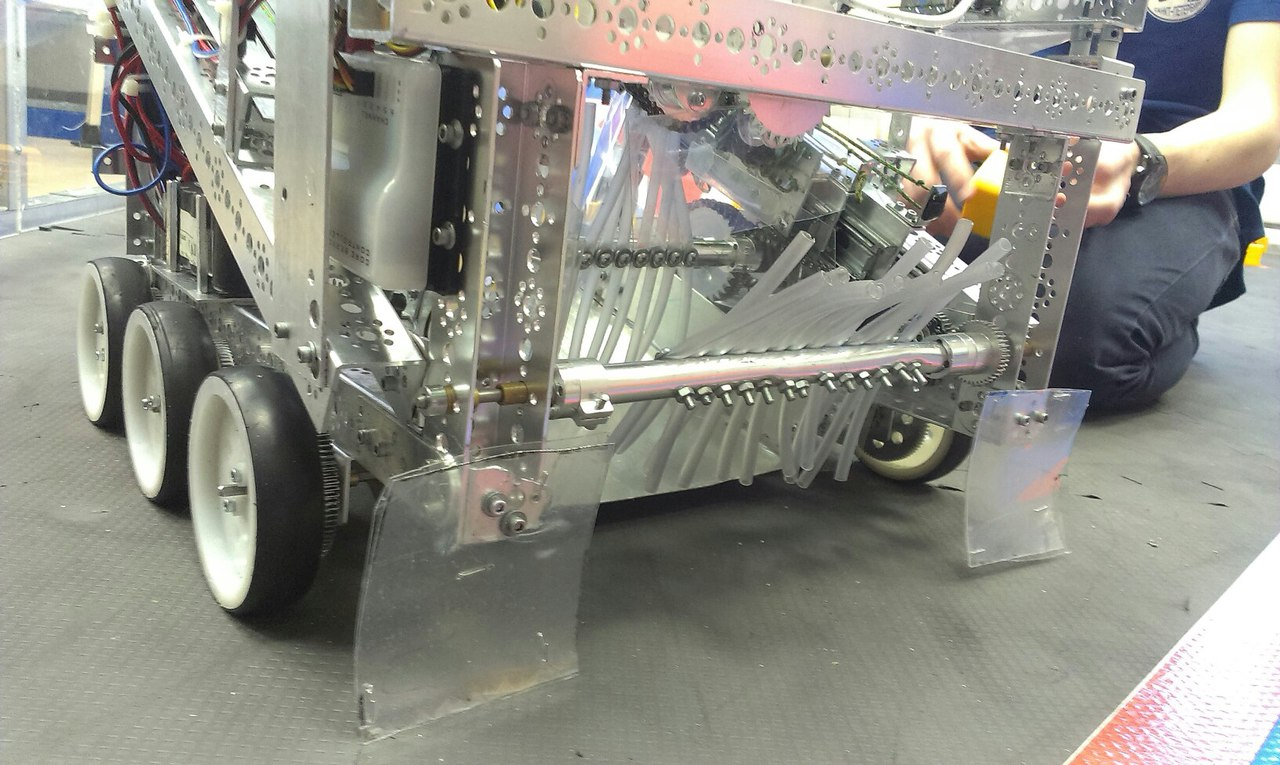
\includegraphics[scale=0.25]{3Engineering/5Team_meetings/days_of_meetings/2016.02.13/images/02}}
		\caption{Protection for wheels}
		\label{Protection1.3}
	\end{minipage}
\end{figure}